\documentclass[twoside,11pt,a4paper,english]{article}

% packages %%%%%%%%%%%%%%%%%%%%%%%%%%%%%%%%%%%%%%%%%%%%%%%%%%%%%%%%%%%%%%%%%%%%
\usepackage{graphicx,curves,float,rotating}

\usepackage{amsmath, amssymb, latexsym}  % math stuff
\usepackage{amsopn}                             % um mathe operatoren zu deklarieren
\usepackage[english]{babel}                     % otherwise use british or american
\usepackage{theorem}                            % instead of \usepackage{amsthm}
\usepackage{dcolumn}
\usepackage{hyperref}
\usepackage[]{algorithm2e}




% @ environment %%%%%%%%%%%%%%%%%%%%%%%%%%%%%%%%%%%%%%%%%%%%%%%%%%%%%%%%%%%%%%%%
\usepackage{xspace}                             % context sensitive space after macros
\makeatletter 
\DeclareRobustCommand\onedot{\futurelet\@let@token\@onedot}
\def\@onedot{\ifx\@let@token.\else.\null\fi\xspace}
\def\eg{{e.g}\onedot} \def\Eg{{E.g}\onedot}
\def\ie{{i.e}\onedot} \def\Ie{{I.e}\onedot}
\def\cf{{c.f}\onedot} \def\Cf{{C.f}\onedot}
\def\etc{{etc}\onedot} \def\vs{{vs}\onedot} 
\def\wrt{w.r.t\onedot} \def\dof{d.o.f\onedot}
\def\etal{{et al}\onedot}
\def\zB{z.B\onedot} \def\ZB{Z.B\onedot}
\def\dh{d.h\onedot} \def\Dh{D.h\onedot}
% %%%%%%%%%%%%%%%%%%%%%%%%%%%%%%%%%%%%%%%%%%%%%%%%%%%%%%%%%%%%%%%%%%%%%%%%%%%%%%%


%	Macros fuer neue Umgebungen
  

%%%%%%%%%%%%%%%%%%%%%%%%%%%%%%%%%%%%%%%%%%%%%%%%%%%%%%%%%%%%%%%%%%%%%%%%%%%%%%
\newcommand*{\Frac}[2]{\frac{\displaystyle #1}{\displaystyle #2}}
\newlength{\textwd}
\newlength{\oddsidemargintmp}
\newlength{\evensidemargintmp}
\newcommand*{\hspaceof}[2]{\settowidth{\textwd}{#1}\mbox{\hspace{#2\textwd}}}
\newlength{\textht}
\newcommand*{\vspaceof}[3]{\settoheight{\textht}{#1}\mbox{\raisebox{#2\textht}{#3}}}
\newcommand*{\PreserveBackslash}[1]{\let\temp=\\#1\let\\=\temp}

\newenvironment{deflist}[1][\quad]%
{  \begin{list}{}{%
      \renewcommand{\makelabel}[1]{\textbf{##1}\hfil}%
      \settowidth{\labelwidth}{\textbf{#1}}%
      \setlength{\leftmargin}{\labelwidth}
      \addtolength{\leftmargin}{\labelsep}}}
{  \end{list}}


\newenvironment{Quote}% Definition of Quote
{  \begin{list}{}{%
      \setlength{\rightmargin}{0pt}}
      \item[]\ignorespaces}
{\unskip\end{list}}


\theoremstyle{break}
\theorembodyfont{\itshape}	
\theoremheaderfont{\scshape}

\newtheorem{Cor}{Corollary}
\newtheorem{Def}{Definition}
%\newtheorem{Def}[Cor]{Definition}



\newcolumntype{.}{D{.}{.}{-1}}


\pagestyle{headings}
\textwidth 15cm
\textheight 23cm
\oddsidemargin 1cm
\evensidemargin 0cm
%\parindent 0mm



%%%%%%%%%%%%%%%%%%%%%%%%%%%%%%%%%%%%%%%%%%%%%%%%%%%%%%%%%%%%%%%%%%%%%%%%%%%%%%%
%
%
%       Jetzt geht's los
%
%
%%%%%%%%%%%%%%%%%%%%%%%%%%%%%%%%%%%%%%%%%%%%%%%%%%%%%%%%%%%%%%%%%%%%%%%%%%%%%%%
\begin{document}


%%%%%%%%%%%%%%%%%%%%%%%%%%%%%%%%%%%%%%%%%%%%%%%%%%%%%%%%%%%%%%%%%%%%%%%%%%%%%%%
%
%
%               Title
%
%
%%%%%%%%%%%%%%%%%%%%%%%%%%%%%%%%%%%%%%%%%%%%%%%%%%%%%%%%%%%%%%%%%%%%%%%%%%%%%%%
\pagestyle{empty}

\begin{center}

    Rheinisch-Westf\"alische Technische Hochschule Aachen \\
    Lehrstuhl f\"ur Informatik 6 \\
    Prof. Dr.-Ing. Hermann Ney\\[6ex]
    Seminar Titel im SS 2018\\[12ex]                          % auch Seminar Titel und Datum �ndern!!!
   
    \LARGE
    \textbf{Deep Clustering for ANN Supported Source Separation } \\[6ex]
    \textit{Patrick von Platen} \\[6ex]
    \Large
    Matrikelnummer 331 430 \\[6ex]
    Datum des Vortrages

    \vfill
    \Large Betreuer: Tobias Menne 
	    
\end{center}

\newpage
\ 
\newpage

%%%%%%%%%%%%%%%%%%%%%%%%%%%%%%%%%%%%%%%%%%%%%%%%%%%%%%%%%%%%%%%%%%%%%%%%%%%%%%%
%
%
%               Inhaltsverzeichnis / Tabellenverzeichnis / Abbildungsverz.
%
%
%
%%%%%%%%%%%%%%%%%%%%%%%%%%%%%%%%%%%%%%%%%%%%%%%%%%%%%%%%%%%%%%%%%%%%%%%%%%%%%%%
\pagestyle{headings}
\tableofcontents
\listoftables
\listoffigures
\newpage
\pagestyle{empty}
\ 
\newpage
\pagestyle{headings}

\section{Introduction} % (fold)
\label{sec:introduction}

When perceiving sound created by multiple acoustic sources, the human auditory system
is extremely good at focussing on parts of the sound coming from only from one acoustic
source.

Imagine yourself at a cocktail party. The sound that you perceive is made up of of all kinds of acoustic sources: The sound of music,
the background chatter of other people talking, the sound of clinking glasses, the 
sound of the person you listening to, etc. Still you can clearly understand the speaker in your group, even though its acoustic signal overlaps at every moment with the acoustic signal of other people speaking and background noise. 

The difficulty of understanding speech in a multiple speaker environment is often called "The cocktail party problem" \cite{CocktailPartyProblem:2000}, first mentioned by Colin Cherry in 1953. 
It was also Colin Cherry, who first brought up the idea of automatic speech separation in his famous paper on experiments of the recognition of speech \cite{Cherry:1953}.
The first method to yield some promising results was introduced by A.S. Bregman in 1990 using \emph{Auditory scene analysis} \cite{bregman1994auditory}.
Since then, multiple methods have been explored. One of them is \emph{Spectral Clustering}
, a method based on partitioning data points into clusters according to eigenstructure
of a similarity matrix. Spectral clustering for source separation earned popularity due
to its ability to find the global maximum \cite{Bach:2006}.

With the rise of deep learning in a variety of applications recently, the first method
to be applied to source separation was presented by Chao Weng and co. in 2015 \cite{SpeechSepDeepLearning:2015}. 
Quickly, different deep learning methods based on a technique called \emph{Deep Clustering} emerged forming the state-of-art in the source separation problem. 
In this report, will focus on the deep clustering method as it was introduced by John R. Hershey and co. in 2015 \cite{BasicDeepClustering:2016} and will study \emph{TasNet}, a deep clustering system performing audio separation in the time domain yielding state-of-the art results \cite{TasNet}.

The applications of automated source separation are wide-ranging. To name a few: 
\begin{itemize}
	\item \textit{Automatic meeting transcription}: In business meetings, multiple speakers are alteranating in a short time or even speaking at the same time. Making it possible to automatically separate speakers from each other and transcribe would be of great use for companies. 
	\item \textit{Virtual assistant}: Virtual assistants, like Alexa, Siri and Google Home are playing a critical part in smart home systems. Filtering out noise and separating the owner's voice from other voices are challenges that can be picked up by automated source separation techniques. 
	\item \textit{Automatic subtitling of music/video}: According to the World Health Organization (WHO) over 5\% of the world population suffers from disabling hearing loss. Subtitling of music and video content, which are often made up of sound coming from multiple acoustic sources, is therefore essential for them \cite{HearingLoss}.	
\end{itemize}

To begin with, the source separation problem is mathematically defined, basic mathematical operations and basic deep learning methods used in deep clustering are explained \ref{sec:basics}.
In the following conventional methods and first attempts of using deep learning techniques for automated source separation are presented \ref{sec:conventional_methods}.
		The essence of this paper being deep clustering and \emph{TasNet} will be presented in-detail in section \ref{sec:deep_clustering_methods}. 
Finally, a conclusion is drawn \ref{sec:conclusion}.
% section introduction (end)

\section{Basics} % (fold)
\label{sec:basics}

This section firstly defines the source separation problem and then gives an 
overview of the most important methods used in systems to tackle it.

\subsection{Definition source separation problem} % (fold)
\label{sec:source_separation_problem}

A generel definition of the source separation problem was given by Jean-Francois Cardoso, 
defininig the problem as ``recovering unobserved signals or sources from several
observed mixtures'' \cite{Cardoso03blindsignal}. He also add two important restrictions that we will apply to our definition as well: 
\begin{enumerate}
 \item the source signals are not observed
 \item no information is available about the mixture
\end{enumerate}

The condition of not even knowing how many sources the mixture is composed of, got coined \emph{blind} source separation \cite{Cardoso03blindsignal}. 
For our purpose, we want to add the restriction of the signal being observed only over a single channel (single microphone).
To sum it up, by talking about the \emph{source separation problem in this paper} is meantto recover the original signals of an unknown amount of sources from a single-channel mixture of the source signals.

To put the above definiton in a mathematical form, let's define: 
\begin{itemize}
	\item the unknown number of acoustic sources: $N$.
	\item the original sound of the i-th source at time t: $x_i(t)$.
	\item the single received sound signal at time t: $X(t) = \sum_{i=1}^{N} x_i(t)$.
\end{itemize}

The goal of source separation is then to recover $x_1(t),...,x_N(t)$ from $X(t)$.
So, defining an algorithm to solve this problem we get:

\begin{algorithm}[ht]
	\RestyleAlgo{boxruled}
	\LinesNumbered
	\textbf{Input: }$X(t)$ \\
	\textbf{Output: }$(N, \{x_1(t), ..., x_N(t)\})$
\end{algorithm}

% section source_separation_problem (end)

\subsection{Mathematical operations} % (fold)
\label{sub:mathematical_oprations}

This subsection aims to shine light on essentiel 
mathematical operations used in the systems that will 
be explained in sections \ref{sec:conventional_methods}, \ref{sec:deep_clustering_methods}. 

\subsubsection{Short term fourier transform} % (fold)
\label{ssub:short_term_fourier_transform}

In order to understand the short term fourier transform, one firstly has to get an understanding of the fourier transform itself. Having a continous signal $s(t)$, the fourier transform is defined as

\[
	S(f) = \int_{\mathbb{R}} s(t) e^{-2j{\pi}ft} dt
\]

The fourier transform $S(f)$ gives the magnitude of every frequency in the signal. A signal can be decomposed as the sum of signals made up of only one frequency (so called sinusoids).
 Thus, one can say that the higher the magnitude of a frequency of the fourier transform, the the higher is the percentage of the signal being composed of the sinusoid of
 this frequency. An important aspect to notice is that the fourier transform of a signal
 integrates over the whole time domain of the signal in order to get the exact magnitude
 of every freuency of the signal. Thus integrating only over a part of the time domain leads
 to approximated values of the frequencies magnitudes. On the other hand, a shorter time
 intervall to integrate over leads to a better time localization of the frequency. This famous
 trade-off is well-known as the uncertainty principle in signal analysis \cite{DBLP:journals/corr/Nam13}.
The short term fourier transform divides the signal into local sections using a window
function $w(\tau) = 0 : \tau \not \in \left[-a, a \right]$ over which the fourier transform is applied.

\[
	S(f,\tau) = \int_{\mathbb{R}} s(t)w(t-\tau) e^{-2j{\pi}ft} dt
\]

It therefore is used to describe the change in frequency over time. Using an appropiate
window funciton leads to a good trade off between time localization and frequency
approximation.

% subsubsection short_term_fourier_transform (end)

\subsubsection{Embedding space} % (fold)
\label{ssub:embedding_space}

An embedding is a structure-preserving, injective mapping $f: X \to Y$. Therefore, every
object of domain $X$ is mapped to a distinct object in domain $Y$ . In this report, we are
interested in embeddings that map to normed spaces meaning that it is possible to measure
the similarity of two objects $x_1$ and $x_2 \in X$ by measuring its distance $d(y_1; y_2) \in \mathbb{R}: y_1, y_2 \in
Y$ .
It is essentially used to convert data to a feature representation where certain properties
can be preserved by distance, so that the data is easily comparable by computers.
One famous example are word embedding models, such as \emph{word2vec} that maps words
to a vector representation. Assuming that words have multiple degrees of similarity, word
embeddings are used to easily calculate the similarity of words on multiple axis \cite{DBLP:journals/corr/abs-1301-3781}.
Later, we will see that the function mapping objects from one domain to an embedding
space can be trained on artificial neural networks and are very powerful tools for the source
separation problem \ref{sec:4.1}.

\subsection{Deep neural network basics} % (fold)
\label{sub:deep_neural_network_basics}

This subsection aims to clarify some deep learning methods and architectures used in the sections \ref{sec:conventional_methods}, \ref{sec:deep_clustering_methods}.

\subsubsection{Recurrent neural network} % (fold)
\label{ssub:recurrent_neural_network}

Recurrent neural networks are neural networks that are ``specialized in processing a sequence
of values $x_1,...,x_t$'' \cite{Goodfellow-et-al-2016}. For that reason, they are very well applicable when dealing
with acoustic signals having high autocorrelation (high correlation between $s(t)$ and
$s(t -� k, s(t + k)$  for $k > 0$).
Recurrent neural networks are extremely effective when dealing with sequential data.
First, recurrent neural networks process data of different time instances in one computation
step, thus taking full advantage of autocorrelation. Second, they can handle data
sequences of variable length in contrast to feed forward neural networks where the input length is determined by the size of the input layer. This is achieved by loops between
recurrent units inside the neural network \cite{Goodfellow-et-al-2016}.
Unfolding a recurrent unit $z$ of a recurrent neural network at different time instances
leads to so-called hidden copies of the network being connected to each other: $z^0, z^1, ..., z^{t-1}, z^{t}$
As a result, such a recurrent unit $z^t$ at time t takes both the output of the node leading
to it ($x^t$) and the output of the same recurrent unit of one time instance earlier $(z^{t-1})$ as input resulting in:

\[
	z^t =f(V x^t + Wz^{t-1} + b)
\]
with $f()$ being the activation function, V the weights between recurrent unit z and input
x, W the weights between two hidden recurrent units $z^{t-1}$ and $z^t$ and b the constant bias term.
This basic setup is known to have the vanishing/exploding gradient problem due to an
exponential decrease/increase in value of long-term components ($\frac{\partial z^t}{\partial z^{t-k}} \to \text{ \textit{const.}} \times W^{k} \to 0 \text{ or } \infty$
)\cite{Pascanu:2013:DTR:3042817.3043083}. To overcome this problem, Hochreiter and co. introduced a ``better'' recurrent unit,
called long shot term memory.

% subsubsection recurrent_neural_network (end)

\subsubsection{Long short term memory} % (fold)
\label{ssub:long_short_term_memory}

To overcome the exploding/vanishing gradients problem, the long short term memory unit
introduces an internal state which can be seen as the unit's ``memory'' \cite{Hochreiter:1997:LSM:1246443.1246450}. At every time
instance t, the unit updates its memory $c^t$ using the memory $c^{t-�}$ and the unit's output
$h^{t-1}$, as well as the new input$x^t$. $c^t$ in combination with $h^{t-1}$ and $x^t$ is then used to
produce the new outputht. The structure of the long short term memory unit is shown in
Figure \ref{fig:lstm}. It is important to notice that the long short term memory uses $x^t$ and $h^{t-1}$ to
compute four different gates: f,i,g,o which are used to control the 
flow of information in
the unit. Also, we can see that when doing backpropagation, the gradient easily ``flows'' to
earlier hidden units without the weight matrix being applied to it (shown by the red arrow) in \ref{fig:lstm}.
This ``highway'' for the gradient strongly reduces the vanishing/exploding gradient
effect and allows the unit to take into account long term dependencies of the input data.

\begin{figure}[h!]
  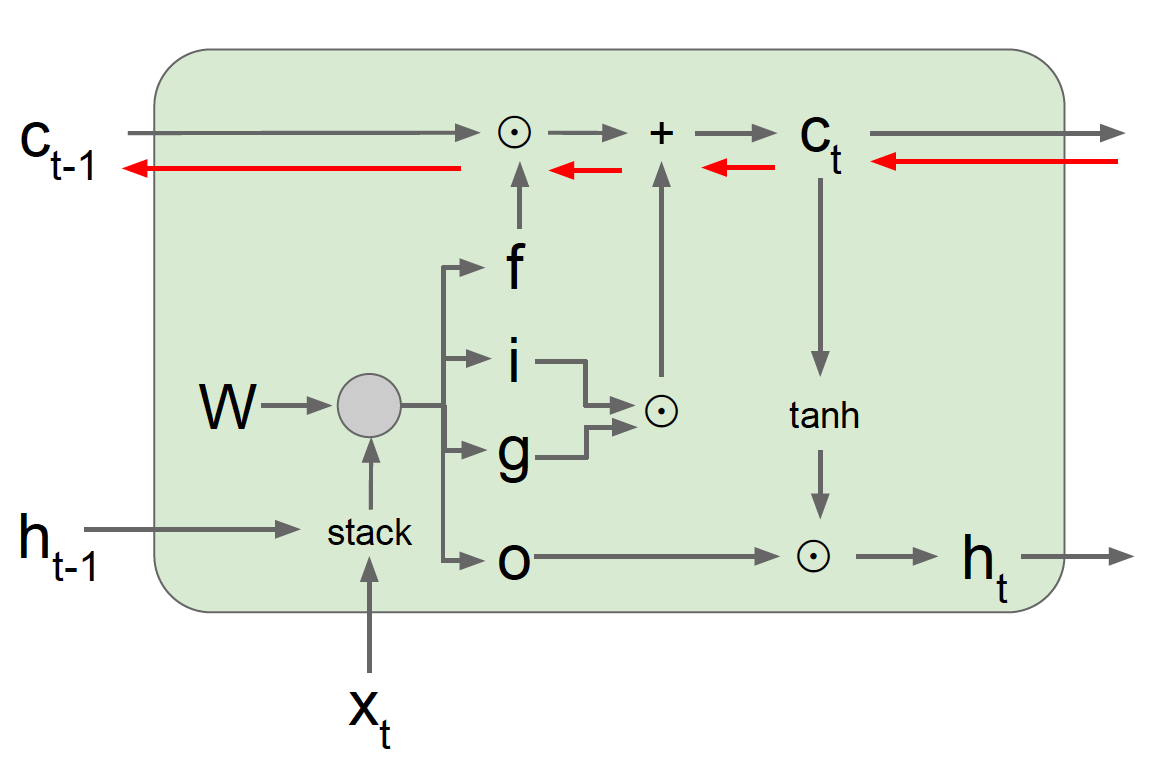
\includegraphics[scale=0.4]{images/lstm_structure.png}
  \centering
  \caption{Long short term memory}
  \label{fig:lstm}
\end{figure}

To furter improve this ability, bi-directional long short term memory units were proposed
to exploit correlations between data in both time directions and are used in many
state-of-the-art systems nowadays. Going more into detail is out of scope for this report,
but more in-detail informationcan be found in \cite{Hochreiter:1997:LSM:1246443.1246450}.

% subsubsection long_short_term_memory (end)

\subsubsection{Autoencoder}

An autoencoder is a neural network that is ``trained to attempt to copy its input to its
output'' \cite{}. It always consists of two parts, the encoder and the decoder. In its simplest
form, the encoder maps the input x to one hidden layer $f(x) = z$ and the decoder tries to
reconstruct the original data $g(z) = x'$ from this layer.
Even though autoencoders are trained with loss functions trying to minimize the difference
between $x$ and $x'$, perfect recontruction of the data input is not the goal. Instead,
autoencoder should be trained in a way preventing them to just copy the input to the
output, but to extract useful information about data distribution instead \cite{Goodfellow-et-al-2016}. Thereby, the
hidden layer should represent the most useful information. Two approaches are considered
in this report.
First, a undercomplete autoencoder is defined by the hidden layer having much lower
dimension than the data, thus forcing the network to ``store all data in a compressed form''.
A backdraw of this approach is that the hidden layer might be two small to learn enough
useful information. Second, a sparse autoencoder forces the hidden layer to be sparse, by
introducing a sparsity penalty on the hidden layer $P(h)$, which will then be added to the
loss function $\mathbb{L}(x,x')+P(h)$. Especially in the field of machine translation, autoencoders
in combination with recurrent neural networks produce state-of-the-art results \cite{DBLP:journals/corr/abs-1801-05119}. 
For more detailed information, please refer to \cite{Goodfellow-et-al-2016}.

% subsection deep_neural_network_basics (end)
% section basics (end)

\section{First attempts using machine learning} % (fold)
\label{sec:conventional_methods}

The first automated metho

\subsection{Spectral Clustering} % (fold)
\label{sub:spectral_clustering}

% subsection spectral_clustering (end)

\subsection{Single-channel Multi-talker separation using deep learning techniques} % (fold)
\label{sub:single_channel_multi_talker_separation_using_deep_learning_techniques}

Present method as explained in \cite{SpeechSepDeepLearning:2015}.

% subsection single_channel_multi_talker_separation_using_deep_learning_techniques (end)

% section conventional_methods (end)

\section{Deep clustering methods} % (fold)
\label{sec:deep_clustering_methods}

I want to present three methods here that more or less can be called deep 
clustering methods and differentiate them between methods using:

\begin{enumerate}
		  \item the (F,T) bins as input -> Frequency Domain Audio Separation Based Methods
			    \item the raw audio signal as input $\to$ Time-Domain Audio Separation Based Methods
\end{enumerate}

Explain challanges:

\begin{itemize}
		  \item Permutation problem 
			    \item Output dimension mismatch problem
\end{itemize}

and state for each method how these challenges can be overcome.

\subsection{Deep clustering method - Frequency domain audio separation based methods} % (fold)
\label{sub:frequency_domain_audio_separation}

Method that assigns contrastive embedding vectors to each time-frequency region.
Present in detail as described in \cite{BasicDeepClustering:2016}.
Can be used for unknown arbitrary amount of sources. 

\subsubsection{Training} % (fold)

Talk about what to pay attention to when training.

\subsubsection{Results} 

talk about what ever

\subsection{TasNet - Time domain audio separation based methods} % (fold)
\label{sub:time_domain_audio_separation}

Introduce TasNet which does not create masks for each source, but instead use encoder-decoder 
framework to model directly the signal in the time-domain. Use \cite{TasNet}.

\subsubsection{Training} % (fold)

Talk about what to pay attention to when training.

\subsubsection{Results}

Talk about results of TasNet

% subsection time_domain_audio_separation (end)
% section deep_neural_network_methods (end)

\section{Conclusion} % (fold)
\label{sec:conclusion}

Write conclusion using results.

\newpage

\addcontentsline{toc}{section}{References}
\bibliographystyle{plain}
\bibliography{vonPlaten_report}

\end{document}
